\documentclass{article}
\usepackage[margin=2cm]{geometry}
\usepackage{graphicx}
\usepackage[pages=some]{background}
\usepackage{titling}
\usepackage{tabularx}
\usepackage{tikz}
\usepackage{forest}
\usepackage{array}
\usepackage{enumitem}
\usepackage{multirow}
\usepackage{subcaption}
\usepackage{float}
\usepackage{amsmath}
\usepackage{amssymb}
\usepackage{multicol}

\forestset{
  my box/.style={
    draw,
    rectangle,
    rounded corners,
    fill=gray!20,
    inner sep=6pt,
    minimum width=3cm % Adjust the width as needed
  }
}

\geometry{a4paper}

\backgroundsetup{
    scale=1,
    angle=0,
    opacity=1,
    contents={%
        
\includegraphics[width=\paperwidth,height=\paperheight]{institution_logo.jpg}
    }
}

\newcommand{\subtitle}[1]{
    \posttitle{
        \par\end{center}
        \begin{center}\large#1\end{center}
        \vskip0.5em}
}

\title{ME-421}
\author{Md. Hasibul Islam}
\subtitle{FLUID MACHINERY}

\begin{document}
\begin{titlepage}
    \centering
    
    {\Huge\bfseries\maketitle}
    \textbf{Quamrul Islam Sir} \\
    \vspace{2cm}
    
\includegraphics[width=8cm]{institution_logo.jpg}
    \vfill
    \vspace*{2cm}
\end{titlepage}

\tableofcontents
\pagebreak
\section{Lecture 01: Introduction} 
\hfill Date: 04/06/2023

\subsection*{Booklist}

\begin{itemize}
    \item Hydraulic Mechanics \hfill \textbf{Govind Rao}
    \item Hydraulic Machines Through worked out problems \hfill \textbf{Published by BUET}
\end{itemize}


\subsection*{Fluid Machines}
The working principle of certain machinery where a fluid is employed to do work.

\subsection*{Components}
Chemically, any petroleum is an extremely complex mixture of hydrocarbon (hydrogen and carbon) compounds with minor amounts of nitrogen, oxygen, and sulfur as impurities. The weight percentage of petroleum is as follows:

\begin{itemize}[label=$\circ$]
    \item Liquid Fluid \footnote{Pump and turbine built together to transmit power smoothly.}
    \begin{itemize}[label=\textendash]
        \item Pumps
        \begin{itemize}[label=\textbullet]
            \item \textbf{Rotodynamics} : Axial flow pump, centrifugal pump etc
            \item \textbf{Positive Displacement} : Reciprocating, gear, screw pump etc
        \end{itemize}
        \item Turbines
        \begin{itemize}[label=\textbullet]
            \item \textbf{Impulse} : Felton wheel (high head)
            \item \textbf{Reaction} : 
            \begin{itemize}[label=\textasteriskcentered]
            		\item Radial Flow
            		\item Mix Flow
            		\item Axial Flow
            \end{itemize}
        \end{itemize}
    \end{itemize}
    \item Gaseous Material
    		\begin{itemize}
    			\item Fans
    			\item Blowers
    			\item Compressors
    			\item Fluid Coupling
    			\item Torque Converter 
    		\end{itemize}
\end{itemize}
\vspace{1cm}
In the case of - 
\subparagraph{Turbines}
Energy is extracted from the fluid to produce torque on a rotating shaft.
\subparagraph{Pumps}
Pump is a device to convert mechanical energy into hydraulic energy.
\\

\subsection*{Pumps}
\subsubsection*{Positive Displacement Type}
Usually consists of one or more chambers which are alternately filled with liquid to be pumped and then emptied again. The rate of discharge depends on the speed of rotation. It takes care relatively small volume of liquid.\\
Example - \textbf{reciprocating pump, gear pump, screw pump} etc

\subsubsection*{Rotodynamics Pump}
In the case of a roto dynamic pump, a rotating element called \textbf{impeller} imparts energy to the liquid and there is a pressure rise.\\
Example - \textbf{centrifugal pump, axial flow pump} etc \\

\subsection*{Reciprocating Pump}

\begin{figure}[H]
  \centering
  \begin{subfigure}[b]{0.4\textwidth}
    \centering
    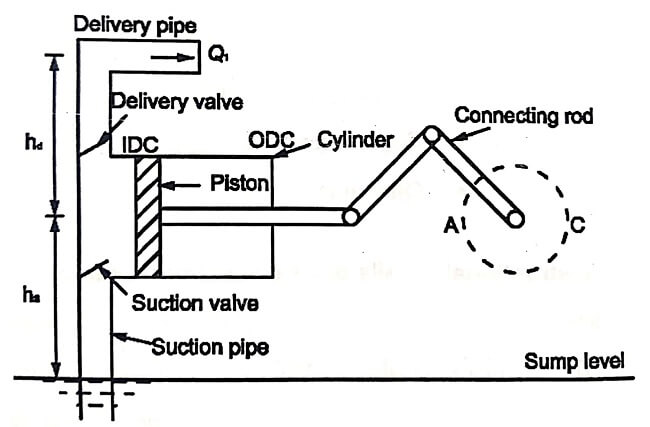
\includegraphics[width=\textwidth]{img/single_acting.jpg}
    \caption{Single Acting Pump}
    \label{fig:image1}
  \end{subfigure}
  \hfill
  \begin{subfigure}[b]{0.4\textwidth}
    \centering
    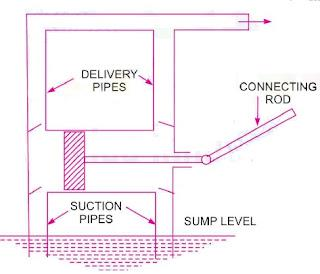
\includegraphics[width=\textwidth]{img/double_acting.jpg}
    \caption{Double Acting Pump}
    \label{fig:image2}
  \end{subfigure}
  \caption{Types of Reciprocating Pump}
  \label{fig:two_images}
\end{figure}

\subsubsection*{Charateristics}
\begin{itemize}
	\item Reciprocating pump is a positive displacement which is driven by power from an external source and consists of a cylinder in which a piston or plunger is blloked backwards and forwards
	\item The movement of the piston or plunger creates alternating vacuum pressure and positive pressure inside the cylinder by means of which water is rised.
	\item If the water acts one side of pistons only, the pump is single acting. If the water acts on both side of the piston, it will suck and deliver during one stroke. such a pump is known as double acting pump.
	\item The reciprocating pump is generally used for producing very high pressure.
	
\end{itemize}

% \newpage
\hrulefill

\section{Lecture 2: Reciprocating Pump}
\hfill Date: 11/06/2023

\subsubsection*{Schamatic diagram of a Reciprocating Pump:}
\begin{figure}[!ht]
  \centering
  \begin{tikzpicture}
    \node[anchor=south west, inner sep=0] at (0,0) {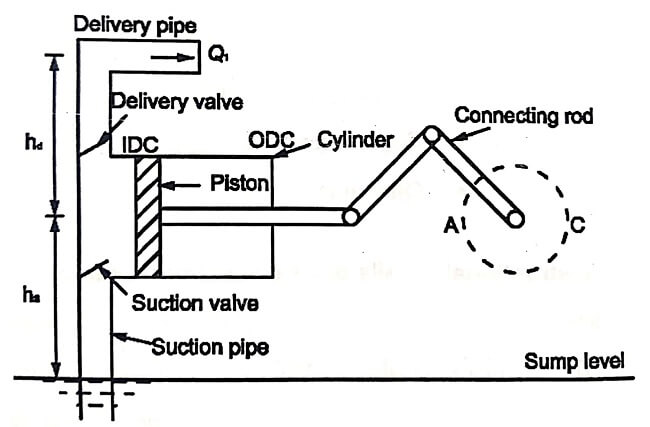
\includegraphics[width=0.75\textwidth]{img/single_acting.jpg}};
  \end{tikzpicture}
  \caption{Schamatic diagram of a Reciprocating Pump}
  \label{fig:reciprocating_pump}
\end{figure}

[Note: Non-return valve, check valve, foot valve -  all are same.]

\subsubsection*{Main Components:}
\begin{itemize}
  \item A piston and a cylinder 
  \item Suction \& delivery valve 
  \item Suction \& delivery pipes 
  \item Crank \& connecting rod 
\end{itemize}


\subsubsection*{Applications:}
The reciprocating pump is best suited for relatively small capacities and high heads. The reciprocating pump is used for - 
\begin{itemize}
  \item Oil drilling operations 
  \item Pneumatic pressure systems 
  \item Feeding small boilers condensate return 
  \item Light oil pumping 
\end{itemize}

\subsubsection*{Operation Principle:}
\begin{itemize}
  \item For a reciprocating pump as crank rotate for piston p moves backwards and forwards with the cylinder c. The piston moves to the right during the suction stroke, which causes vaccum in the cylinder. 
  \item The atmospheric pressure under sump (reservoir) water surface forces the water up the suction pipe. 
  \item The suction valve a is opened and water enters into the cylinder. The delivery valve b remains closed.
  \item During the return stroke of the piston, the water pressure closes the suction valve and opens the delivery valve b. Water is then forced up the delivery pipe and raised to the required height or pressure. 
  \item For a single acting pump, the theoretical volume of water raise per revolution is equal to the stroke volume of the cylinder and twice this volume is, if the pump is double acting. 
\end{itemize}

\subsubsection*{Coefficient of Discharge, $C_d$:}
It is the ratio of actual volume of water discharge to the volume swept by the piston. \\

\[ C_d = \frac{{\text{{actual discharge per stroke}}}}{{\text{{volume swept per stroke}}}} \]

\subsubsection*{Slip :}
Slip is the difference between actual discharge and theoretical discharge. 

\[ Slip = Q_t - Q_a\]
\begin{align*}
  \text{where,} \quad &Q_t \text{→ Theoretical Discharge} \\
  \text{and} \quad &Q_a  \text{→ Actual Discharge}
\end{align*}

\[ {\text{percentage slip}} = \frac{Q_t - Q_a}{Q_t} \times 100 \] 


\subsubsection*{Negative Slip:}
In case of a reciprocating pump with long suction pipe, short delivery pipe and running at high speed, inertia force in the suction pipe becomes large as compared to the pressure force on the outside of delivery valve. This opens the delivery valve even before the piston has completed its suction stroke. Some of the water is pushed into the delivery pipe before the delivery stroke is actually commenced. The actual discharge will be more than the theoretical discharge and slip will be negative. The coefficient of discharge will be greater than 1. 

\subsubsection*{Problem 01:}
The actual discharge of a single acting reciprocating pump is 0.02 $m^3/s$, when running at 55 rpm. The length of the stroke is 500 mm and diameter of the piston is 250 mm. For a total static heads of 16 m, calculate the percentage slip, coefficient of discharge and power required to drive the pump.\\ 

\textbf{Solution:}\\
Given data : \\ 
\begin{tabular}{ll}
  Actual Discharge, $Q_a$ & = 0.02 $m^3/sec$ \\
  Speed of the pump, N & = 55 rpm \\
  Stroke Length, L & = 500 mm\\
  Diameter of piston, d & = 250 mm \\
  Total static head, $H_{st}$ & = 16 m\\ 
\end{tabular} \\
Find - (a) Percentage Slip, (b) Coeff. of discharge, (c) Power required to drive the pump.\\

\begin{align*}
  \text{Cross sectional area of piston, A} &= \frac{\pi}{4}  \times d^2 \\
  &= \frac{\pi}{4} \times (0.25)^2 \, m^2 \\
  &= 0.0491 \, m^2
\end{align*}

\begin{align*}
  \text{Theoretical Discharge, } Q_t &= \frac{L \times A \times N}{60}\\
  &= \frac{0.5 \times 0.0491 \times 55}{60} \, m^3/sec \\
  &= 0.0225 \, m^3/sec
\end{align*}

\begin{align*}
  \text{Percentage slip } &= \frac{Q_t - Q_a}{Q_t} \times 100\\
  &= \frac{0.0225 - 0.02}{0.0225} \times 100 \\
  &= 11.10\% \\
\end{align*}

\begin{align*}
  \text{Coefficient of Discharge, } C_d &= \frac{Q_a}{Q_t} \\
  &= \frac{0.02}{0.0225} \\
  &= 0.89 \\
\end{align*}

\begin{align*}
  \text{Power required to drive the pump } &= Q_t \times \gamma \times H_{st}\\
  &= 0.0225 \times 9800 \times 16 \, watt \\
  &= 3.53 \, kW \\
\end{align*}
\hrulefill

\section{Lecture 3: Flow Rate and Work Done}
\hfill Date: 18/06/2023

\begin{multicols}{2}
  let, \\
  r = crank radius \\
  L = Length of stroke = 2r \\ 
  A = Cross Sectional Area of Piston \\
  N = RPM \\
  \\
  $H_s$ = Suction Head \\
  $H_d$ = Delivery Head \\
  $\gamma$ = Specific weight of water \\
\end{multicols}

Volume of water supplied in one stroke = $AL$ \\
Theoretical flow rate per second, $Q$ = $\frac{LAN}{60}$ \\
For a double acting pump discharge = $\frac{2LAN}{60}$ \\
W = weight flow rate = $Q\gamma$ \\
Total height lifted, H = $H_s + H_d$ \\
Theoretical power required to drive the pump = $Q \gamma \left(H_s + H_d\right) = WH$\\
The actual power required will be greater than the theoretical power due to friction, leakage etc.

\subsection*{Indicator diagram of a reciprocating pump:}
Indicator diagram may be defined as the graphical representation of pressure head in the cylinder and the volume swept by piston for one complete revolution.  
\begin{figure}[h]
  \begin{center}
    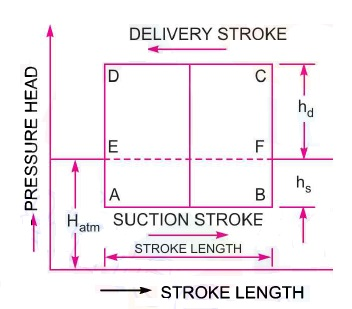
\includegraphics[width=0.7\linewidth]{img/indicator_diagram.jpg}
    \caption{Indicator diagram of a reciprocating pump.}
  \end{center}
\end{figure}

  In the above figure, shows the theoretical indicator diagram of a reciprocating pump under an ideal conditions (without friction and leakage). The stroke length and pressure head inside the cylinder are represented by x and y axis in the diagram respectively. 

  \begin{multicols}{2}
    In the diagram,\\
    $H_d$ = Delivery Head \\
    $H_s$ = Suction Head \\ 
    Line $ef$ = Represents atmospheric pressure \\
    Line $ab$ = Represents pressure inside the cylinder during suction stroke \\
    Line $cd$ = Represents pressure inside the cylinder during delivery stroke \\
    \\
    x-axis = absolute zero pressure \\
    area $abfe$ = Work done by  the piston dring suction stroke \\
    area $cdef$ = work done by the piston during delivery stroke \\
  \end{multicols}

  \subsection*{Variation of Pressure due to acceleration of piston }
  \begin{figure}[h]
    \begin{center}
      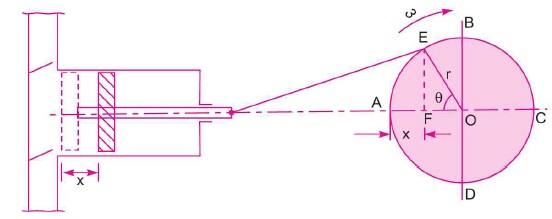
\includegraphics[width=0.7\linewidth]{img/acceleration_piston.jpg}
      \caption{Variation of Pressure due to acceleration of piston}
    \end{center}
  \end{figure}
  Due to reciprocating motion of the piston, there will be acceleration at the beginning and retardation at the end of each stroke. For this reason, the inertia of water will cause a variation in the pressure in the cylinder.

  \subsubsection*{Assumption}
  \begin{itemize}
    \item Length of the connecting rod is very large 
    \item The rotation of the crank is uniform 
    \item The piston makes simple harmonic motion 
  \end{itemize}

  \subsubsection*{Nomenclature}

  \begin{multicols}{2}
    A = Cross sectional area of piston \\
    a = Cross sectional area of pipe \\
    $\omega$ = Angular velocity of rotating crank \\
    r = crank radius \\
    \\
    l = Total length of pipe \\
    $\gamma$ = specific weight of water \\
    $v$ = velocity of water in a pipe \\
    $V$ = velocity of piston \\
  \end{multicols}

  \subsubsection*{Derivation of Equation}
  Let, adter time t, the crank makes an angle $\theta$ with horizontal. Therefore, $$\theta = \omega \times t$$
  Displacement of piston in time t, $x = r -r \cos \theta = r - r \cos \left(\omega t\right)$

  Velocity of piston in time t, $v$ = $\frac{dx}{dt} = r\omega \sin \left(\omega t\right)$

  acceleration of piston in time t, $f$ = $\frac{dv}{dt} = r\omega^2 \cos \left(\omega t\right)$

  From continuity equation, \\
  Cross sectional area of pipe $\times$ velocity of water in pipe = Velocity of pison $\times$ cross sectional area of piston \\
  i.e., $av = AV$ \\
  or, $v = \frac{A}{a} V = \frac{A}{a} r \omega \sin \omega t = \frac{A}{a} r \omega \sin \theta $

  Acceleration of water in pipe = $\frac{dv}{dt} = \frac{A}{a} r \omega^2 \cos \omega t = \frac{A}{a} \omega^2 r \cos \theta$ 

  weight of water in pipe = $\gamma a l$ \\ 
  mass of water in pipe = $\frac{\gamma a l}{g}$

  let, $P_a$ = intensity of pressure due to acceleration of water in pipe \\
  from newton's second law of motion,\\
  Force = Mass $\times$ Acceleration \\
  $$P_a \times a = \frac{\gamma a l}{g} \frac{A}{a} \omega^2 r \cos \theta$$
  \begin{equation}
    P_a = \frac{\gamma l}{g} \frac{A}{a} \omega^2 r \cos \theta \label{eq:eq1}
  \end{equation}

  Let, $H_a$ = acceleration pressure head 
  =$\frac{\text{intensity of pressure}}{\text{specific weight of water}} = \frac{P_a}{\gamma}$

  Dividing the equation (1) by $\gamma$ we have,
  $$\frac{P_a}{\gamma} = \frac{l}{g} \frac{A}{a} \omega^2 r \cos \theta$$
  \begin{equation}
    H_a = \frac{l}{g} \frac{A}{a} \omega^2 r \cos \theta \label{eq:eq2}
  \end{equation}

  From equation (2) it is found that pressure head due to acceleration vary with the angle $\theta$. \\
  At the beginning of stroke, $\theta = 0, cos\theta = 1$ \\
  $$\therefore H_a = \frac{l}{g} \frac{A}{a} \omega^2 r$$ 

  At the middle of stroke, $\theta = 90, cos\theta = 0$ \\
  $$\therefore H_a = 0$$ 

  At the end of stroke, $\theta = 180, cos\theta = -1$ \\
  $$\therefore H_a = - \frac{l}{g} \frac{A}{a} \omega^2 r$$ 
  $\checkmark$ here (-ve) means retardation.

  \hrulefill 

  \section{Lecture 4: Indicator diagram \& Air Vessel}
\hfill Date: 09/07/2023

\subsubsection*{Problem}
The and stroke of a double acting pump are 250mm and 300 mm respectively. The pump discharge is 0.038 $m^3/s$ of water at 50 rpm. Through a portal static head of 12m. Find the ship and actual power required to drive the pump with 80\% efficiency. 

\subsubsection*{Solution}

\begin{multicols}{2}[Given Data]
  Bore diameter, d = 350 mm \\
  Stroke length, L = 300 mm \\
  Speed, N = 50 rpm \\ 
  Total Static Head, $H_{st}$ = 12 m \\
  Actial discharge, $Q_a$ = 0.038 $m^3/s$ \\
  Pump efficiency, $\eta$ = 80\% 
  
\end{multicols}

Find:\\
 - Slip of the pump \\
 - Power Required to drive the pump \\

Cross sectional area of cylinder, $A = \frac{\pi}{4} d^2 = 0.096 m^2$ \\
Theoretical discharge, $Q_t = \frac{2LAN}{60} = 0.048 m^3/s$ \\
Slip of the pump = $Q_t - Q_a = 0.048 - 0.038 = 0.01 m^3/s$ \\ 

Power Required to drive the pump, $P = \gamma Q_t H_{st} = 5.65 kW$

Efficiency, $$\eta = \frac{\text{theoretical power}}{\text{actual power}}$$
$$\Rightarrow 0.8 = \frac{5.65}{\text{actual power}}$$
$$\Rightarrow \text{actual power} = 7.063 kW $$ 
\hspace*{0.65\linewidth}(ans:)

\subsubsection*{Important Note}
Actual power will be more than theoretical power due to friction, weight, auxiliary back flow and others.


\subsection*{Separation}
It has been experimentally found that when the vaccum pressure head ($H_s + H_a$) reaches 7.9 m of water or 2.4 m absolute. The continuity of flow will stop because of water will commenced vaporized and the separation of flow will take place, therefore to avoid separation, 
$$H_s + H_a = 7.9 m$$ 

\begin{itemize}
  \item If water temperature is higher, it can not be pumped by creating vaccum. Rather it will be vaporized. 
\end{itemize}


\subsection*{Indicator Diagram with Acceleration Head}
\begin{figure*}[h]
  \begin{center}
    \includegraphics*[width=0.7\linewidth]{img/indicator_dia.jpeg}
    \caption*{Indicator diagram with acceleration head}
  \end{center}
  \end{figure*}

\begin{enumerate}
  \item The acceleration head, $H_a$ is added to the vaccum head at the beginning of suction stroke and subtracted at the end.
  \item In the delivery stroke, the acceleration head, $H_a$ is added at the beginning of the delivery strooke and subtracted at the end. 
  \item The inertia of water doesn't affect the net work done, but only causes a variation of pressure in the cylinder.  
\end{enumerate}

  \subsection*{Air Vessel in a Reciprocating Pump}
  \begin{figure*}[h]
    \begin{center}
      \includegraphics*[width=0.7\linewidth]{img/air_vessel.jpeg}
      \caption*{Air Vessel in a Reciprocating Pump}
    \end{center}
    \end{figure*}

    \subsubsection*{Definition}
    An air vessel is a cast iron chamber which has an openning at the base through which water can flow.

    \subsubsection*{Characteristics}
    \begin{enumerate}
      \item Volume of air vessel is 5-9 times of pump displacement volume. 
      \item The vessel is filled with compressed air with opening at it's base. 
      \item The vessels are fitted in suction and delivery pipe close to the cylinder. 
    \end{enumerate}

    \section{Lecture 5: Problems on Reciprocating Pump}
    \hfill Date: 16/07/2023

    \begin{multicols*}{2}
      \subsubsection*{Problem-01}
      A double acting reciprocating pump has a 500 mm diameter and stroke of 500 mm respectively. The pump is required to deliver 0.1 $m^3/s$ water at a head of 100 m. Frictional losses are estimated to be 1 m in suction pipe and 19m in delivery pipe. Velocity of water in delivery pipe is 1 m/s. Overall efficiency is 85\% and slip is 3\%. Determine the speed of the pump and power required for the pump. 

      \subsubsection*{Solution:} 
      Given data:\\
      \begin{align*}
        &\text{Cylinder diameter, } d = 500 \text{ mm} \\
        &\text{Stroke length, } L = 500 \text{ mm} \\
        &\text{Actual discharge, } Q_a = 0.1 \text{ m}^3/\text{s} \\
        &\text{Static head, } H_s + H_d = 100 \text{ m} \\
        &\text{Frictional losses in suction pipe, } h_{fs} = 1 \text{ m} \\
        &\text{Frictional losses in delivery pipe, } h_{fd} = 19 \text{ m} \\
        &\text{Velocity of water in delivery pipe, } v_d = 1 \text{ m/s} \\ 
        &\text{Overall efficiency, } \eta_o = 85\% \\
        &\text{Percentage slip} = 3\%  
      \end{align*}
      Slip = $\frac{Q_t - Q_a}{Q_t} \times 100\% \Rightarrow Q_t = 0.1031 \, m^3/s $   \\
      Theoretical discharge, $Q_t = \frac{2LAN}{60} \Rightarrow  N = 31.51 \, rpm $  \\
      Total head against which the pump has to work, \\
      $H = H_s + H_d + h_{fs} + h_{fd} + \frac{v^2}{2g} = 120.05 \,m$ \\
      Overall efficiency,$\eta_o = \frac{\text{Theoretical power}}{\text{actual power}}$ \\
      Actual power = 142.8 kW  

      \subsubsection*{Problem-02}
      A single acting reciprocating pump running at 45 rpm as a piston of diameter 150 mm and stroke length of 200 mm. The suction pipe diameter is 150 mm and it's length is 20 m. Determine the acceleration head at the beginning of suction stroke. 
      \subsubsection*{Solution:}
      Given data:
      \begin{align*}
        &\text{Piston diameter, d} = 150 mm \\
        &\text{stroke length, L} = 200 mm \\
        &\text{suction pipe diameter,} d_s = 150 mm \\
        &\text{suction pipe length }, l_s = 20 m \\
        &\text{Speed of pump,} N = 45 rpm 
      \end{align*}
      
      At the beginning of suction stroke, $\theta = 0,  \cos \theta = 1$ \\
      Angular velocity, $\omega = \frac{2\pi N}{60} = 5.3014$ rad/s \\
      Crank radius, r = $\frac{L}{2} = 100 mm$ \\
      Cross sectional area of piston, A = $\frac{\pi}{4} (0.15)^2$ \\ 
      Cross sectional area of pipe, a = $\frac{\pi}{4} (0.15)^2$\\
      Acceleration head, $$H_a = \frac{l_s}{g} \frac{A}{a} \omega^2 r \cos \theta = 4.52 \, m $$

      \subsubsection*{Problem-03}
      Single acting reciprocating pump as a bore of 500 mm and a stroke of 500 mm respectively. The pump delivers 0.11 $m^3/s$ water against a head of 100 m. The head loss due to friction in suction and delivery pipe are 2 m  and 14 m respectively. The velocity of water in pipe is 1.5 m/s. If the pump efficiency is 92\% and slip is 5\%. Calculate the speed of the pump and power required to drive the pump. 

      \subsubsection*{Solution:}
      Given data: \\
      \begin{align*}
        &\text{Cylinder diameter, } d = 500 \text{ mm} \\
        &\text{Stroke length, } L = 500 \text{ mm} \\
        &\text{Actual discharge, } Q_a = 0.11 \text{ m}^3/\text{s} \\
        &\text{Head, } H = 100 \text{ m} \\
        &\text{Frictional losses in suction pipe, } h_{fs} = 2 \text{ m} \\
        &\text{Frictional losses in delivery pipe, } h_{fd} = 14 \text{ m} \\
        &\text{Velocity of water in delivery pipe, } v_d = 1.5 \text{ m/s} \\ 
        &\text{Overall efficiency, } \eta_o = 92\% \\
        &\text{Percentage slip} = 5\%  
      \end{align*}
      Slip = $\frac{Q_t - Q_a}{Q_t} \times 100\% \Rightarrow Q_t = 0.116 \, m^3/s $   \\
      Theoretical discharge, $Q_t = \frac{2LAN}{60} \Rightarrow  N = 70.89 \, rpm $  \\
      Total head, \\
      $H_t = H + h_{fs} + h_{fd} + \frac{v^2}{2g} = 116.11 \,m$ \\


      Overall efficiency,$\eta_o = \frac{\text{Theoretical power}}{\text{actual power}}$ \\
      Actual power = 143.47 kW  

      \subsubsection*{Problem-04}
      Single acting reciprocating pump running at 45 rpm as a piston of diameter of 150 mm and the stroke length of 200 mm. The suction pipe is 150 mm diameter and of length 20 m. Determine the maximum possible suction head to avoid separation. 

      [Formula: $H_s + H_a = 7.9$]

      \subsubsection*{Solution:}
      Given data:
      \begin{align*}
        &\text{Piston diameter, d} = 150 mm \\
        &\text{stroke length, L} = 200 mm \\
        &\text{suction pipe diameter,} d_s = 150 mm \\
        &\text{suction pipe length }, l_s = 20 m \\
        &\text{Speed of pump,} N = 45 rpm 
      \end{align*}

      Crank radius, r = $\frac{L}{2} = 100 mm$ \\
      Cross sectional area of piston, A = $\frac{\pi}{4} (0.15)^2$ \\ 
      Cross sectional area of pipe, a = $\frac{\pi}{4} (0.15)^2$\\
      Acceleration head, $$H_a = \frac{l_s}{g} \frac{A}{a} \omega^2 r \cos \theta = 4.527 \, m $$
      
      To avoid separation,
      $$H_s + H_a = 7.9 \, m$$
      $$\Rightarrow H_s = 3.37 \, m$$
    \end{multicols*}
\end{document}
